\documentclass[5pt]{ltjsarticle}
\usepackage{luatexja-otf}
\usepackage[]{luatexja,luatexja-fontspec}\usepackage{booktabs}
\usepackage{array}
\usepackage{graphicx}
\usepackage{mathpazo}
\usepackage{amsmath}
\usepackage{amsthm}
\usepackage{amssymb}
\usepackage{amsfonts}
\usepackage[noheadfoot,top=10mm,bottom=10mm,hmargin=10mm]{geometry}
\usepackage{tikz}
\usetikzlibrary{matrix}
\usepackage{pgfcore}
\usepackage{color}
\usepackage{longtable}
\newtheorem{dfn}{Def}
\newtheorem{thm}{Thm}
\newtheorem{cor}{Cor}
\newtheorem{prop}{Prop}
\newtheorem{rk}{remark}
\newtheorem{claim}{claim}
\newtheorem{recall}{recall}
\newtheorem{ques}{Q.}
\date{\today}
\author{俺}
\title{テスト}
\begin{document}\maketitle
\section{関手}

\subsection{関手とは}

\begin{itemize}
\item
  圏の間の射に相当するもの
\item
  写像をモチーフに定義されている

  \begin{itemize}
  
  \item
    写像は集合環に定義されるものだが、今は簡単のため大きなクラスの間の写像的対応も写像と呼ぶことにする
  \end{itemize}
\item
  一般に、共変関手と反変関手という二種類の分類がある
\end{itemize}

以下、\(\mathbf{A},\mathbf{B}\)を圏とする。

\subsection{定義と例}

\dfn{共変関手の公理}

写像\(F:\mathbf{A} \to \mathbf{B}\)が\textbf{共変関手}であるとは次が成り立つことを言う:

\(\forall f \in \mathbf{A}.\)

\begin{enumerate}

\item
  \(F(\Box f) = \Box F(f)\)
\item
  \(F(f \Box) = F(f) \Box\)
\item
  \(F(fg) = F(f) F(g)\ \ \ \ \text{ただし} f \Box = \Box g\)
  公理の見取り図を に示す。
\end{enumerate}

\begin{itemize}
\item
  {[}※{]}対象上の写像と射集合の間の写像として定義する本が多いが、対象を恒等射と同一視すれば純粋に射の間の写像として定義される
\item
  {[}※{]}恒等射を恒等射に写すことから、対象上の写像は射の写像の内容に含まれている
\end{itemize}

参考までに、対象の写像と射の写像として定義した場合は次の感じになる:

\begin{enumerate}
\item
  \(\forall A \in \mathbf{A} (F(A) \in \mathbf{B})\)
\item
  \(\forall A,B \in \mathbf{A} (F:(A,B) \to (F(A),F(B));f \mapsto Ff\text{は写像})\)
\item
  \(\forall A \in \mathbf{A} (F(1_A) = 1_{F(A)})\)
\item
  \(\forall f,g \in \mathbf{A} (F(fg) = F(f)F(g))\ \ \ \ \text{ただし}f\Box = \Box g\)
\end{enumerate}

\dfn{反変関手の公理}

\(F:\mathbf{A} \to \mathbf{B}\)が \textbf{反変関手}
であるとは次が成り立つことを言う:

\(\forall f \in \mathbf{A}\) 1. \(F(\Box f) = F(f)\Box\)

\begin{enumerate}

\item
  \(F(f\Box) = \Box F(f)\)
\item
  \(F(fg) = F(g)F(f)\)
\end{enumerate}

射の始域と終域が逆転するところが共変関手と異なる。

佐藤君に上目遣いでしゃぶらせたい

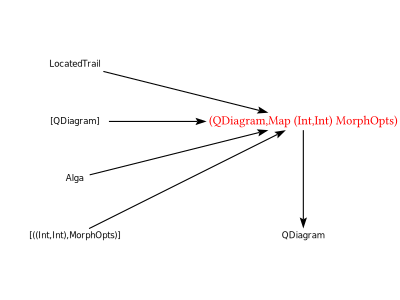
\includegraphics{test.pdf}
\end{document}
